\chapter{FUNDAMENTAÇÃO TEÓRICA}
\label{chap:fundamentacaoTeorica}

\section{VIRTUALIZAÇÃO}
\label{sec:virtualizacao}

Virtualização, basicamente, é a técnica de separar aplicação e sistema operacional dos componentes físicos. Por exemplo, uma máquina virtual possui aplicação e sistema operacional como um servidor físico, mas estes não estão vinculados ao software e pode ser disponibilizado onde for mais conveniente. Uma aplicação deve ser executada em um sistema operacional em um determinado software. Com virtualização de aplicação ou apresentação, estas aplicações podem rodar em um servidor ou ambiente centralizado e ser deportada para outros sistemas operacionais e hardwares.

\subsection{\textit{HYPERVISOR}}
\label{sec:hypervisor}

O \textit{hypervisor} é um \textit{firmware} ou hardware que cria e roda máquinas virtuais (\textit{VMs}). O computador no qual o \textit{hypervisor} roda uma ou mais VMs é chamado de máquina hospedeira (\textit{host}), e cada \textit{VM} é chamada de máquina convidada (\textit{guest}). O \textit{hypervisor} se apresenta aos sistemas operacionais convidados como uma plataforma de virtualização e gerencia a execução dos sistemas operacionais convidados. 

Existem dois tipos de hypervisor, o primeiro tipo é conhecido como bare matal, onde o próprio sistema operacional que gerencia as VM, podemos citar o VMware: ESX, Xem, CubeOS, Microsoft Hyper-V. O segudo modelo é o hosted onde o hypervisor se encontra encima do sistema operacional, seja Linux, Windowns ou MacOS, podemos citar o virtualbox, VMware: Workstation, QEMU, OVirt.   

\subsection{VIRTUALIZAÇÃO COMPLETA E PARCIAL}
\label{sec:virtualizacao-completa-parcial}

Como o próprio nome sugere, a virtualização completa realiza toda a abstração do sistema físico, com o objetivo de fornecer ao sistema operacional hóspede uma réplica do hardware  virtualizado pelo hospedeiro. Este tipo dispensa a necessidade de modificar o SO convidado, que trabalha desconhecendo que há virtualização.

Com a virtualização total, as instruções não críticas são executadas diretamente no hardware, enquanto as instruções críticas são interceptadas e executadas pela hypervisor. O sistema operacional visitante, no entanto, sequer tem o conhecimento de que está sendo executado sobre o hypervisor.

Já um SO convidado paravirtualizado tem a assistência de um compilador inteligente que atua na substituição de instruções de SO não virtualizáveis por hiperchamadas (hypercalls) quando for executar uma instrução sensível. Tal procedimento poupa o desempenho, quando comparado ao que foi descrito na virtualização total.

Em relação aos dispositivos de E/S, a paravirtualização permite que as máquinas virtuais usem os drivers do dispositivo físico real sob o controle do hipervisor, o que reduz os problemas de compatibilidade.

\section{CONTAINER LINUX}
\label{sec:linux-countainer}

A \citeonline{redhat1} define o que ẽ um container Linux em seu artigo "O que é um container Linux?" como:
\begin{citacao}
	Um container Linux é um conjunto de um ou mais processos organizados isoladamente do sistema. Todos os arquivos necessários à execução de tais processos são fornecidos por uma imagem distinta. Na prática, os containers Linux são portáteis e consistentes durante toda a migração entre os ambientes de desenvolvimento, teste e produção. Essas características os tornam uma opção muito mais rápida do que os pipelines de desenvolvimento, que dependem da replicação dos ambientes de teste tradicionais.
\end{citacao}  

Imagine que você esteja desenvolvendo uma aplicação. Você trabalha em um laptop, e o seu ambiente tem uma configuração específica. Outros desenvolvedores podem ter configurações um pouco diferentes. A aplicação é baseada nessa configuração e depende de bibliotecas, dependências e arquivos específicos. Ao mesmo tempo, a empresa em que você trabalha possui ambientes de desenvolvimento e de produção padronizados com uma configuração própria, e também possui seus próprios conjuntos de arquivos auxiliares. Você deseja emular esses ambientes localmente, sem a necessidade de recriar os ambientes do servidor. Então, como fazer a aplicação funcionar em ambientes diferentes, ser aprovada pela garantia de qualidade e implantá-la sem muito esforço, sem a necessidade de reescrever ou realizar reparos no código? A resposta é: containers.

\begin{figure}[!htb]
	\centering
	\caption{Container}
	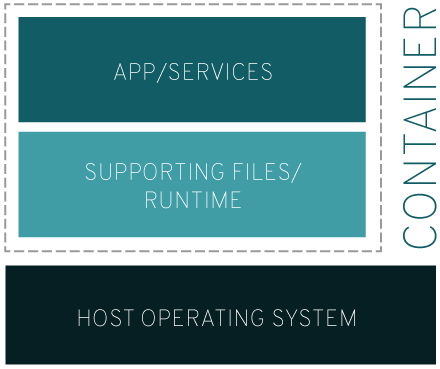
\includegraphics[width=0.5\textwidth]{figuras/what-is-a-container.png}
	\fonte{\citeonline{redhat1}}
	\label{fig:figura-exemplo1}
\end{figure}

O container que abriga a aplicação tem as bibliotecas, as dependências e os arquivos necessários para migrá-la por todos os ambientes até a produção, sem os efeitos colaterais indesejados. Na verdade, você deve imaginar o conteúdo de uma imagem de container como uma instalação de uma distribuição do Linux, pois essa imagem é completa com pacotes RPM, arquivos de configuração e outros elementos. No entanto, é muito mais fácil lidar com uma distribuição de imagem de container do que instalar novas cópias de sistemas operacionais. Dessa forma, evita-se o conflito e todos ficam satisfeitos.

\subsection{EVOLUÇÃO DOS CONTAINERS}

Os conteiners não surgiram no Linux, mas surgiu inicialmente no FreeBSD em 2000 como jails, essa tecnologia ê capaz de particionar um sistema FreeBSD em vários subsistemas ou celas (por causa disso o nome "jails" ). Eles foram desenvolvidos para serem ambientes seguros que podiam ser compartilhados entre os membros de equipe ou colegas de trabalho. Os jails tem como propósito, criar processos em um ambiente isolado utilizando o chroot ("Changing root" ou trocando a raiz), que consiste em mentir para os processos, para achar que a raiz ou o começo do sistema de arquivos está em uma determinada pasta, fazendo eles percam o acesso ao sistema de arquivos real. Um sistema operacional inteiro rodado  de maneira isolada a partir de uma pasta.  Contudo a implementação estava incompleta e com o tempo foram descobertos métodos de escapar do ambiente em jail. 

Logo após, foram implementadas no Linux os grupos de controle (cgroups) que limita o uso de recursos por um processo ou grupo de processos. Com a mudança do sistema de inicialização padrão do sysV para systemd, que possui uma melhor integração com o cgroups, possibilitou ter mais controle sobre os processos isolados. Ambas as tecnologias, além de adicionarem um controle geral ao Linux, serviram como estrutura para a separação eficaz de ambientes.

Com os avanços em namespaces de kernel, pode-se virtualizar, desde IDs de processos a nomes de rede. E os namespaces de usuários “permitem realizar mapeamentos de IDs de usuários e grupos por namespace. No que diz respeito a containers, isso faz com que os usuários e grupos podem ter privilégios para executar determinadas operações dentro de um container, sem ter esses mesmos privilégios fora dele. Por conta disso surgiu o projeto Linux Containers (LXC) que melhorou a experiência do usuário na utilização de containers, contribuindo com ferramentas para facilitar a inicialização de containers com uma interface de linha de comando simples.

Porém, mesmo com os avanços do LXC, estava longe de ser amigável com o publico. Com isso surgiu o docker, mudando completamento a forma de criar, gerenciar, compartir, depurar e de iniciar containers. Levando a tecnologia de containers a outro patamar, sendo utilizado pelas maiores impressas no mundo. 

\section{CONTAINER ENGINE}
\label{sec:countainerEngine}

Em 2008, o Docker entrou em cena (por meio do dotCloud) com sua tecnologia de container homônima. A tecnologia Docker adicionou muitos dos novos conceitos e ferramentas: uma interface de linha de comando simples para executar e criar novas imagens em camadas, um daemon de servidor, uma biblioteca de imagens de container pré-criadas e o conceito de servidor de registros. Combinadas, essas tecnologias possibilitaram aos usuários criar novos containers em camadas com rapidez e compartilhá-los facilmente com outras pessoas.

A Red Hat reconheceu o poder da colaboração nesse novo ecossistema e usou a tecnologia subjacente no nosso OpenShift Container Platform. Para afastar o receio de haver um único fornecedor controlando uma tecnologia tão importante, a Docker Inc. contribuiu com muitos dos componentes subjacentes utilizados em projetos open source realizados pela comunidade (o runc faz parte da Open Containers Initiative (OCI) e o containerd foi transferido para o CNCF).

Há três padrões principais que garantem a interoperabilidade das tecnologias de containers: as especificações Image, Distribution e Runtime da OCI. A combinação dessas especificações permite que projetos da comunidade, soluções comerciais e provedores de cloud criem tecnologias de container interoperáveis (por exemplo, pense em uma situação em que você precisa introduzir imagens personalizadas no servidor de registro do provedor de cloud). Atualmente, a Red Hat e a Docker, juntamente com muitas outras organizações, são membros da Open Container Initiative, cujo objetivo é padronizar as tecnologias de containers no setor open source.

\begin{figure}[!htb]
	\centering
	\caption{LXC vs container}
	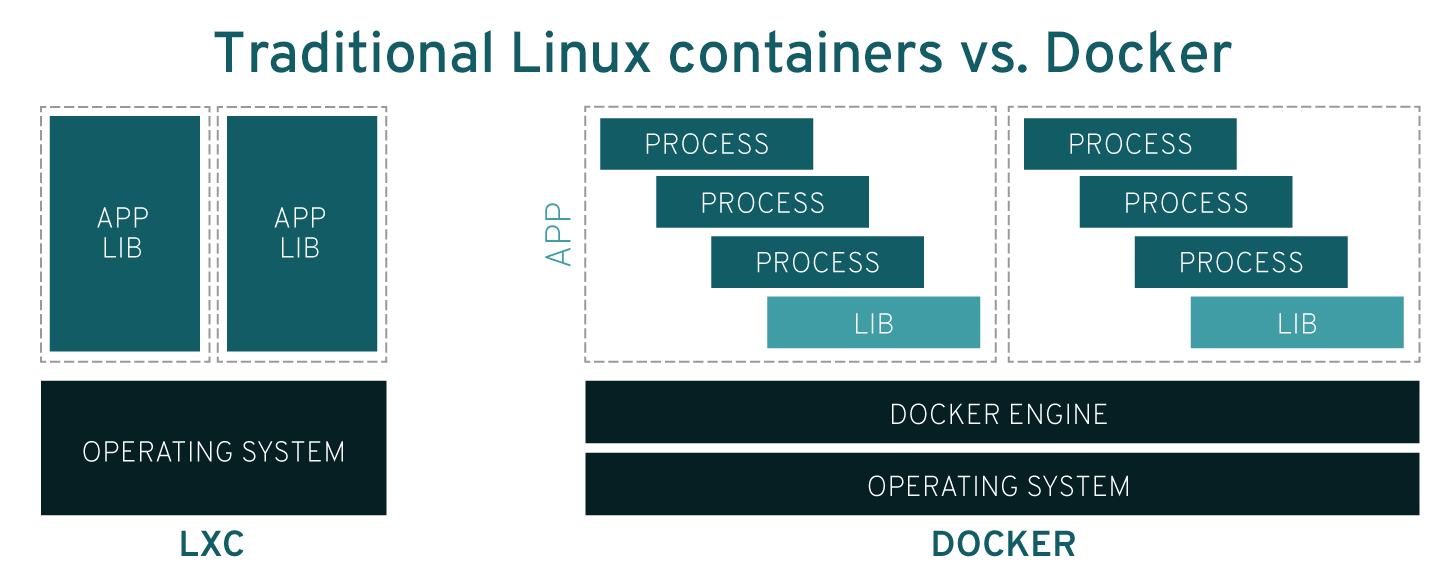
\includegraphics[width=0.9\textwidth]{figuras/traditional-linux-containers-vs-docker_0.png}
	\fonte{\citeonline{redhat1}}
	\label{fig:lxc-vs-containers}
\end{figure}

\section{VIRTUALIZAÇÃO VS CONTAINER}
\label{sec:virtualização-vs-container}
As duas tecnologias são complementares. Aqui está uma maneira fácil de distinguir ambas:

Com a virtualização, é possível executar sistemas operacionais (Windows ou Linux) simultaneamente em um único sistema de hardware.

Os containers compartilham o mesmo kernel do sistema operacional e isolam os processos da aplicação do restante do sistema. Por exemplo: os sistemas ARM Linux executam containers ARM Linux, os sistemas x86 Linux executam containers x86 Linux e os sistemas x86 Windows executam containers x86 Windows. Os containers Linux são extremamente portáteis, mas devem ser compatíveis com o sistema operacional subjacente.

O que isso significa? Para começar, a virtualização usa um hipervisor para emular o hardware, o que permite executar vários sistemas operacionais simultaneamente. Essa não é uma solução tão leve quanto o uso de containers. Quando a capacidade e os recursos são limitados, é necessário usar aplicações leves que possam ser implantadas densamente. Os containers Linux são executados de maneira nativa no sistema operacional, compartilhando-o com todos os outros containers. Assim, as aplicações e os serviços permanecem leves e são executados em paralelo com agilidade.

Os containers Linux são mais um salto evolucionário no desenvolvimento, implantação e gerenciamento de aplicações. Com as imagens de containers Linux, é possível ter portabilidade e controle de versão. Assim, isso ajuda a garantir que os trabalhos contidos no laptop do desenvolvedor sejam executados corretamente no ambiente de produção. Em comparação com as máquinas virtuais, executar containers Linux consome menos recursos, oferece uma interface padrão (início, interrupção, variáveis de ambiente etc.), mantém a aplicação isolada e facilita o gerenciamento dos processos, como parte de uma aplicação maior (vários containers). Além disso, é possível orquestrar as aplicações em vários containers em diversas clouds.

\begin{figure}[!htb]
	\centering
	\caption{Virtualização vs container}
	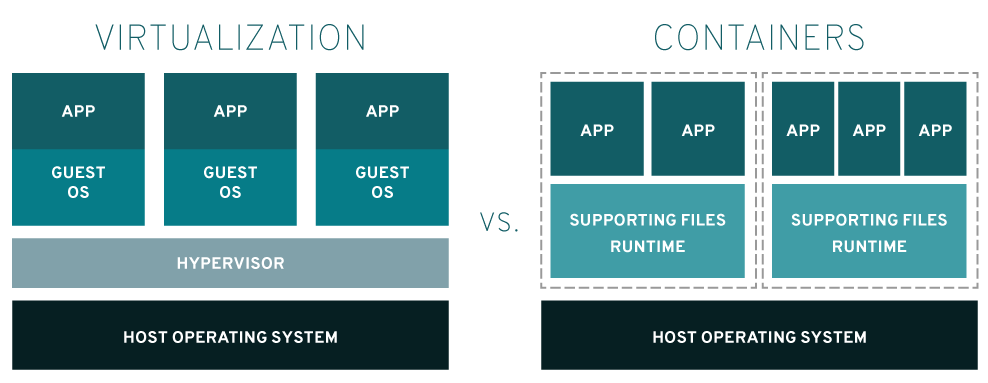
\includegraphics[width=0.9\textwidth]{figuras/virtualization-vs-containers.png}
	\fonte{\citeonline{redhat1}}
	\label{fig:virtualization-vs-containers}
\end{figure}



